\chapter{Guida utente}

\section{Installazione ed Esecuzione}

Per installare ed eseguire il Progetto, bisogna prima di tutto eseguire la \textbf{Build} tramite Shell, attraverso il seguente comando: 
\begin{verbatim}
    sbt clean pack
\end{verbatim}
Successivamente si pu\`o procedere con l'esecuzione, eseguendo prima il comando che permette al \textbf{Server} di avviarsi:
\begin{itemize}
    \item Windows: \begin{verbatim}
    ./server/target/pack/bin/amongsus-server
\end{verbatim}
    \item Linux/Mac \begin{verbatim}
    .\server\target\pack\bin\amongsus-server
\end{verbatim}
\end{itemize}
Ed infine il comando che permette di eseguire il gioco:
\begin{itemize}
    \item Windows: \begin{verbatim}
    ./client/target/pack/bin/app-launcher
\end{verbatim}
    \item Linux/Mac \begin{verbatim}
    .\client\target\pack\bin\app-launcher
\end{verbatim}
\end{itemize}
Qui di seguito rappresentiamo alcune schermate del gioco:

\begin{figure}[ht]
\centering
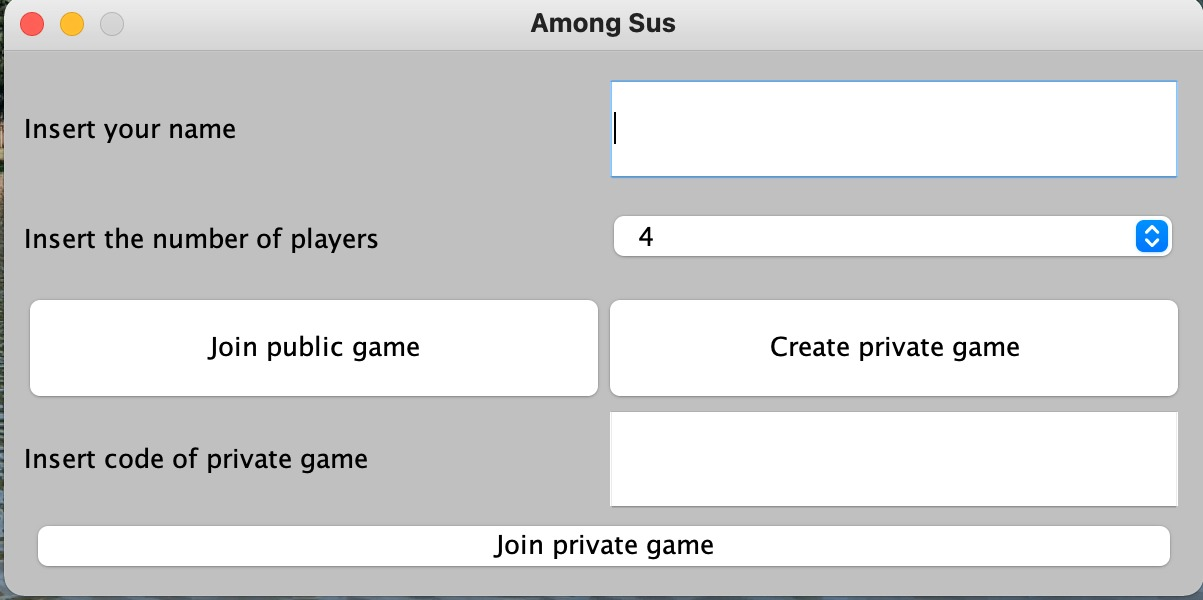
\includegraphics[width=10cm, height=6.5cm]{img/menu-frame.jpeg}
\caption{Men\`u iniziale} 
\end{figure}

\begin{figure}[ht]
\centering
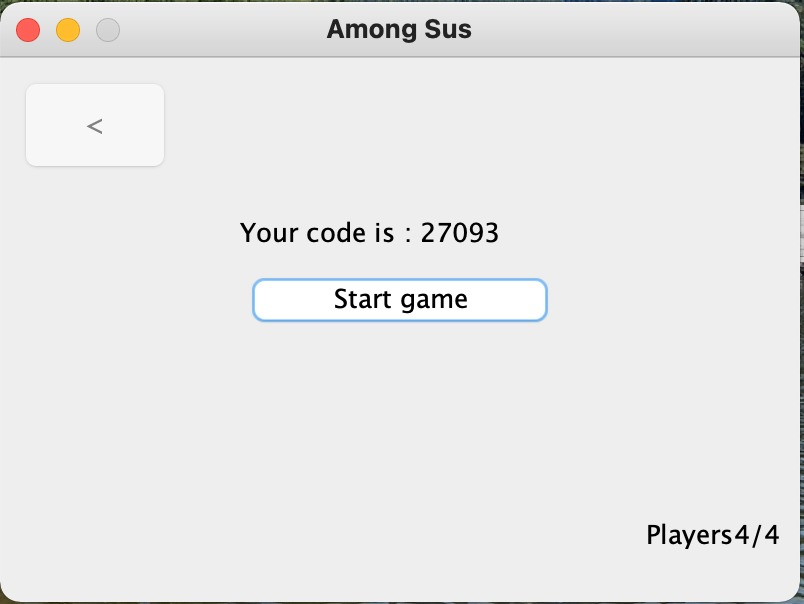
\includegraphics[width=10cm, height=7cm]{img/lobby-frame.jpeg}
\caption{Lobby partita privata}
\end{figure}

\begin{figure}[ht]
\centering
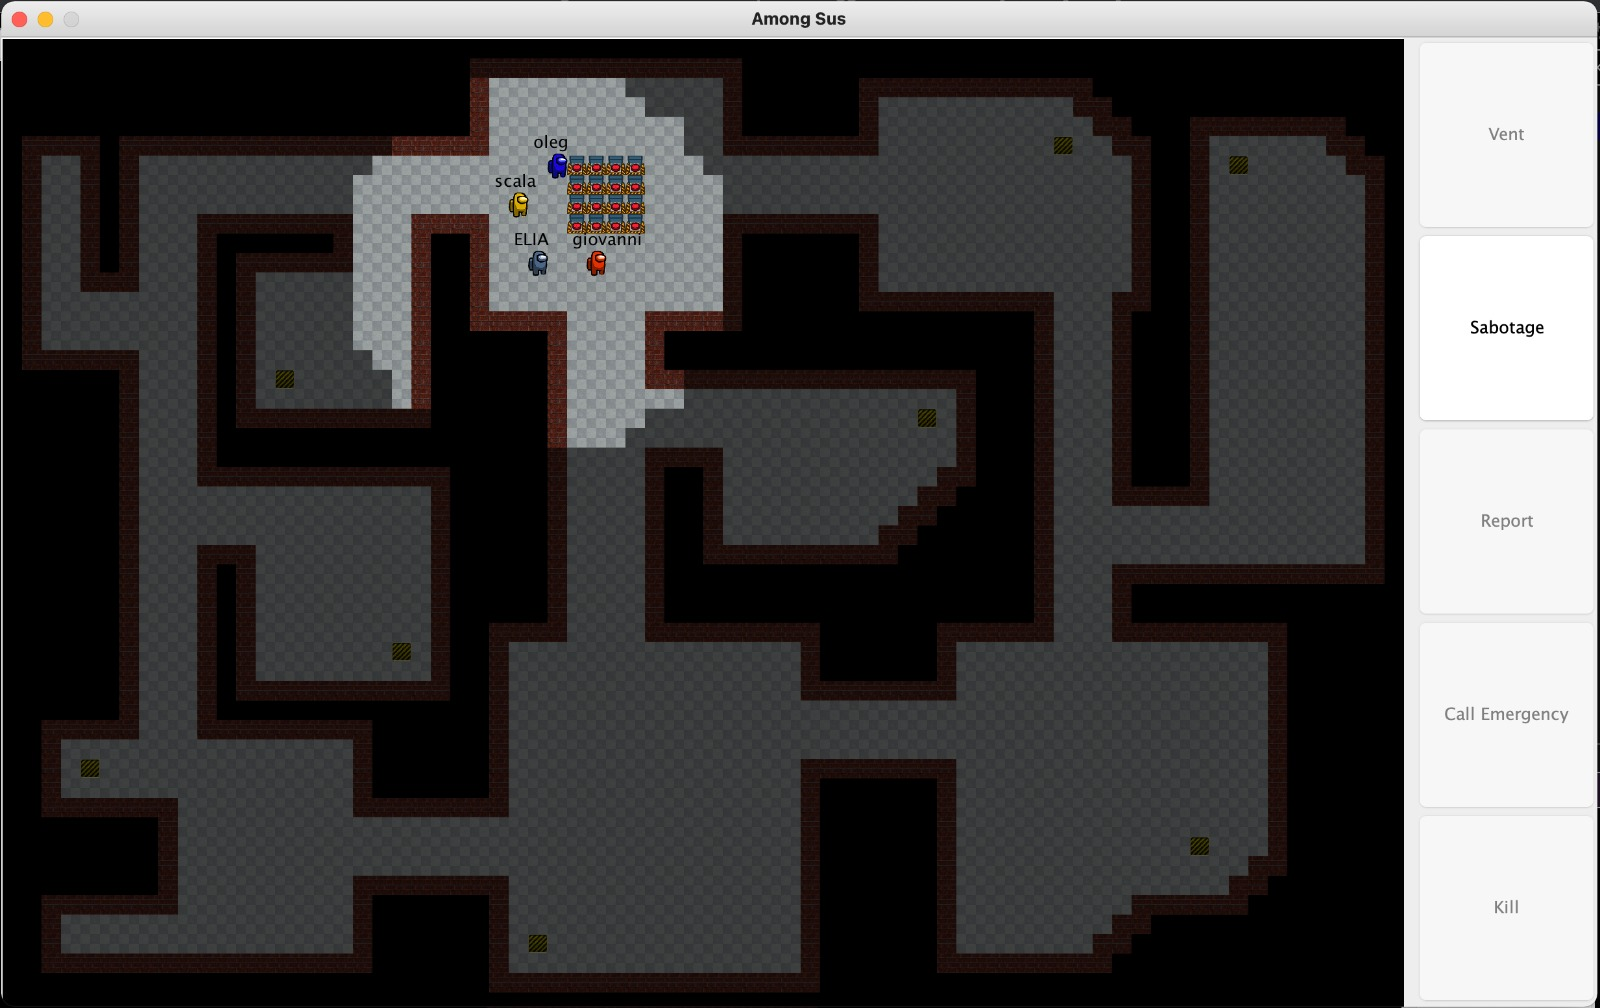
\includegraphics[width=12cm, height=8cm]{img/impostor-game.jpeg}
\caption{Partita con ruolo Impostore}
\end{figure}

\begin{figure}[ht]
\centering
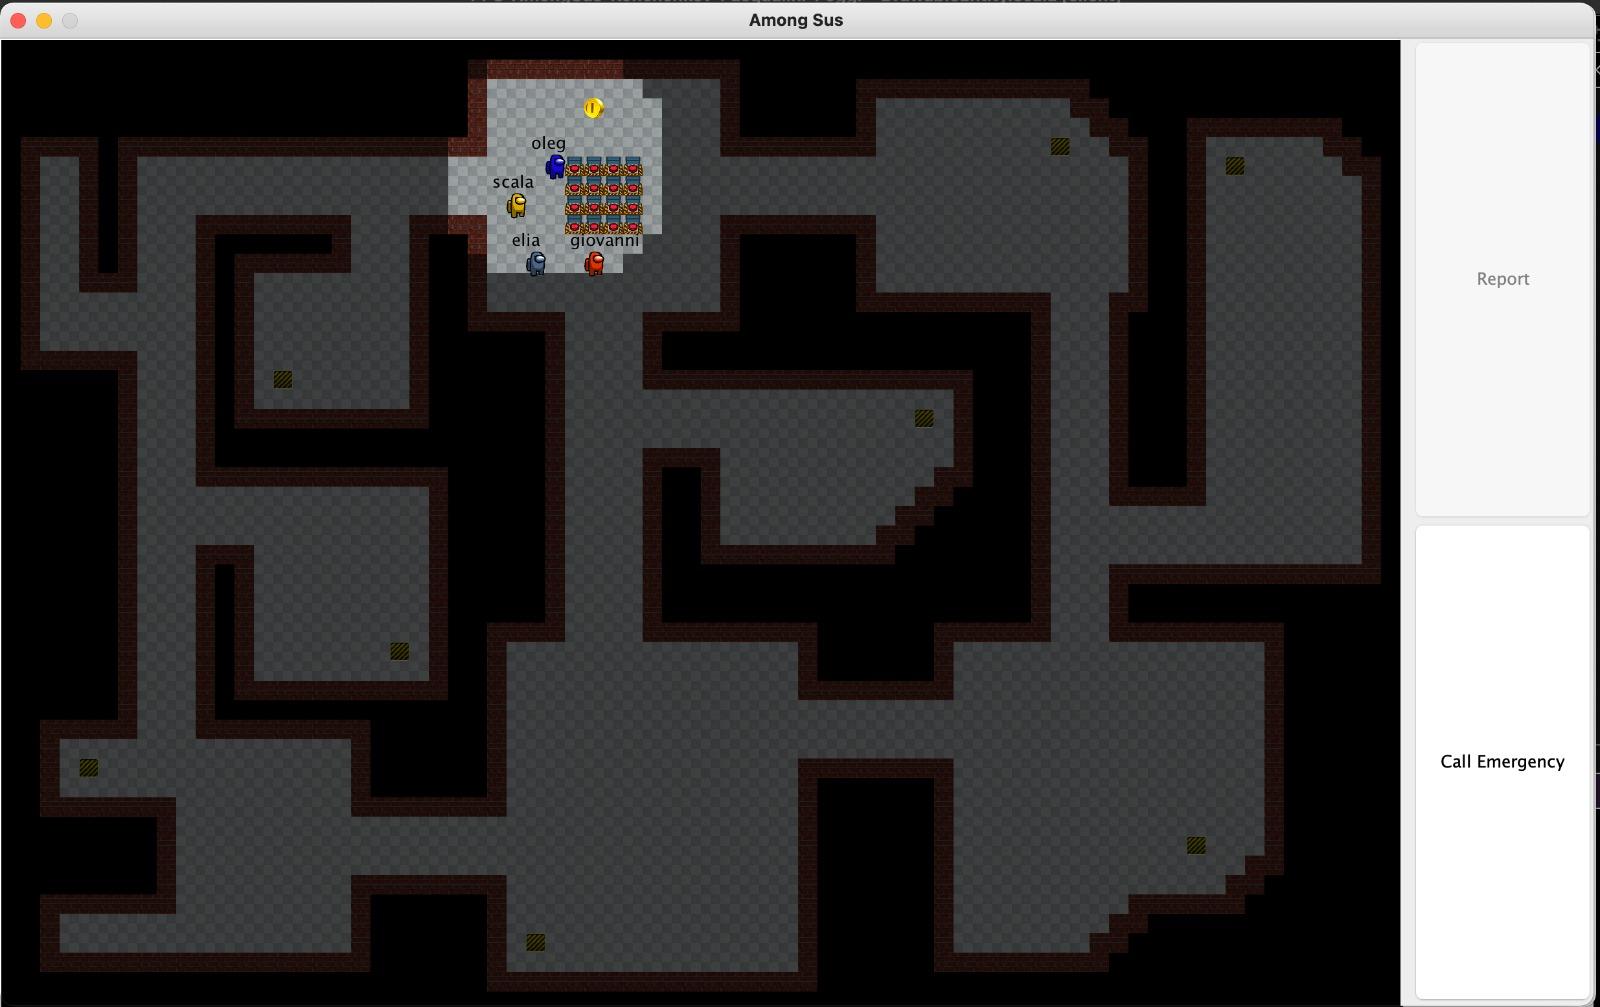
\includegraphics[width=12cm, height=8cm]{img/crewmate-game.jpeg}
\caption{Partita con ruolo Crewmate}
\end{figure}